%!TEX root = main_mestrado.tex
\chapter{Contexto}
\label{ch:contexto}

Neste capítulo descrevemos qual a finalidade e como funcionam comunidades de perguntas e respostas. Ademais, focando na plataforma \emph{StackExchange}, descrevemos sua história, estrutura, além de como são dispostos os perfis dos usuários.
% Descrição geral do capítulo

\section{Comunidades de Perguntas e Respostas} % (fold)
\label{sec:comunidades_de_perguntas_e_respostas}
Dentre os vários sites e comunidades que se propuseram a formar um banco de informações online e disponível à toda internet, comunidades de perguntas e respostas têm se destacado por serem um meio social e colaborativo para formar tal depósito de conhecimento.

Sites como \emph{Quora}, \emph{Yahoo! Answers} e as comunidades do \emph{StackExchange} são exemplos de sucesso de tais comunidades. E, apesar do design e das abordagens diferentes, todas têm o mecanismo de funcionamento similar: usuários postam perguntas que são expostas publicamente e divididas por tópicos ou \emph{tags}. Outros usuários, então, podem responder tais perguntas e suas respostas recebem votos pelo questionador e demais membros da comunidade, como um controle de qualidade.

Tais sites atraem milhões de usuários passivos (conhecidos como \emph{lurkers}) e ativos que, sem recompensa financeira alguma, são responsáveis por todo o conteúdo gerado por estes sites e que também é disponibilizado à comunidade sem custo algum. Tal conteúdo é considerado como confiável e com um nível de qualidade não esperado para um site cujo conteúdo é produzido por qualquer pessoa que se voluntarie, fazendo com que essas comunidades e seu conteúdo sejam consideradas um forte atrativo para pesquisadores.

% section comunidades_de_perguntas_e_respostas (end)

\section{\emph{StackExchange}}

Com mais de 100 sites sobre assuntos diversos, o \emph{StackExchange} não se trata apenas de uma comunidade de perguntas e respostas, mas de uma plataforma. Apesar de se destacar nas comunidades relacionadas à \emph{STEM}, o \emph{StackExchange} possui sites nos mais diversos assuntos, desde viagens, passando por culinária e chegando até a comunidades dedicadas a línguas e religiões como alemão e islamismo. A Tabela~\ref{table:categories} mostra um resumo com as categorias de comunidades presentes na plataforma \emph{StackExchange}, a quantidade de sites em cada categoria e a idade média dos sites em cada categoria.
% O que é o StackExchange

\begin{table}[h]
\centering
\begin{tabular}{@{}ccc@{}}
\toprule
{\small\textit{Categoria}} & {\small \textit{Comunidades}} & {\small \textit{Idade (meses)}} \\ \midrule
business           & 3  & 43 \\
culture-recreation & 21 & 39 \\
life-arts          & 15 & 44 \\
professional       & 2  & 25 \\
science            & 12 & 43 \\
technology         & 32 & 47 \\ \bottomrule
\end{tabular}
\caption[Resumo das categorias do \emph{StackExchange}]{Esta tabela apresenta o número de comunidades por categoria e a média das idades das comunidades de cada categoria, em meses.}~\label{table:categories}
\end{table}

\subsection{História} % (fold)
\label{sub:hist_ria}
% Como surgiu o StackExchange

Tudo começou com o site \emph{StackOverflow}, que foi criado em 2008 por dois engenheiros de software chamados Joel Spolsky e Jeff Atwood, com o intuito de ser uma alternativa a fóruns voltados para programadores, que costumavam ser populares na época. Com seu design diferenciado, o \emph{StackOverflow} foi cativando a comunidade, atraindo centenas de usuários e, no ano seguinte, mais duas comunidades foram criadas pelos mesmos criadores do \emph{StackOverflow}, para suprir a demanda por sites similares focando em assuntos não relacionados à programação de computadores: \emph{ServerFault} e \emph{SuperUser}.

A plataforma StackExchange foi lançada publicamente no início de 2011, já contando com 33 sites sobre diversos temas. Hoje, a plataforma conta com 144 comunidades, divididas em seis categorias: Tecnologia, Cultura, Artes, Ciência, Negócios e Profissional. Com mais de cinco milhões de usuários cadastrados e centenas de milhares de visitas por dia, o \emph{StackExchange} cresceu muito desde 2008, mas sua comunidade mais popular continua sendo a \emph{StackOverflow}~\cite{wikipedia:stackexchange,wikipedia:stackoverflow}.

% subsubsection hist_ria (end)

\begin{figure}[!b]
  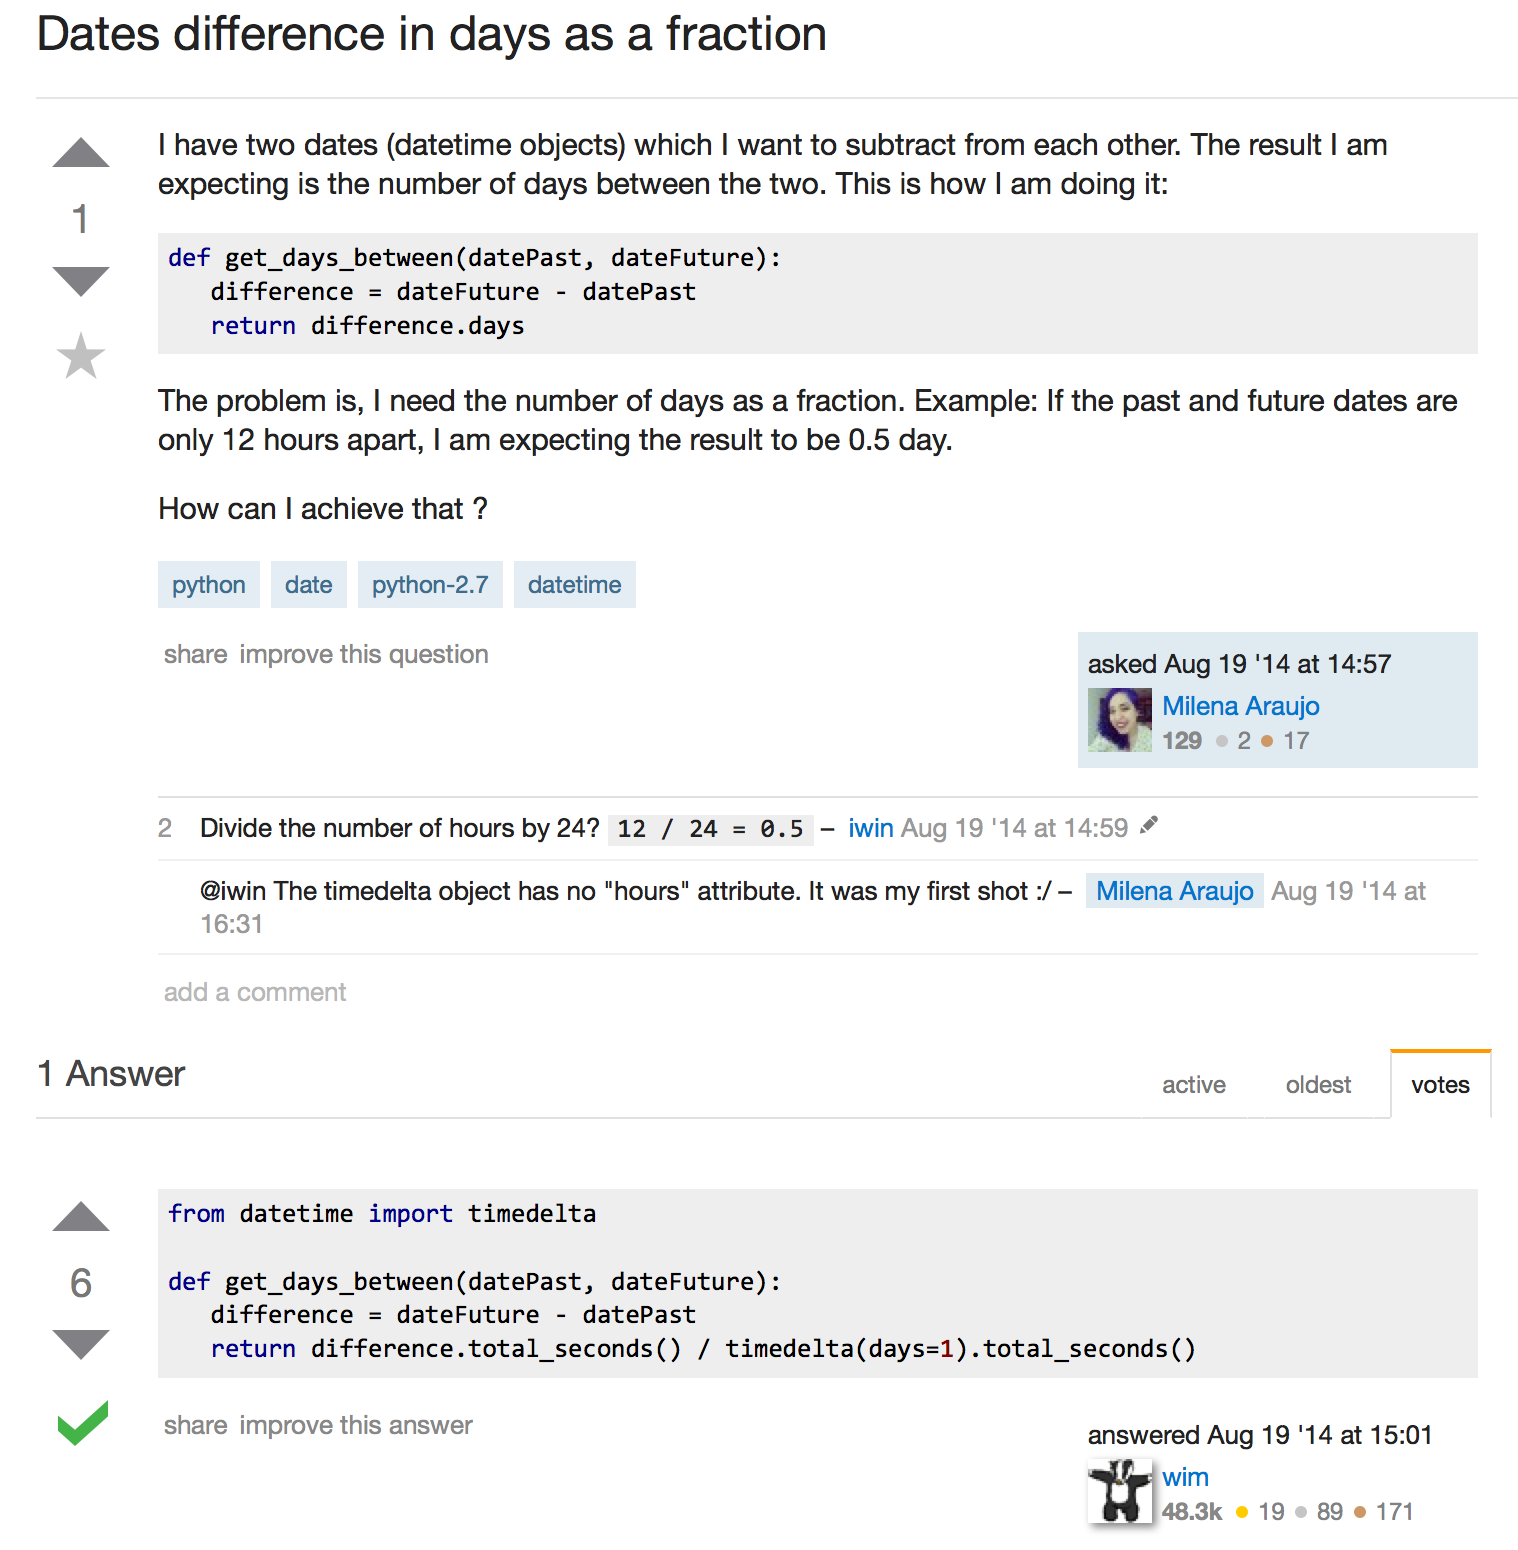
\includegraphics[width=1\columnwidth]{figures/post.png}
  \caption[Exemplo de uma página de pergunta no \emph{StackOverflow}]{Exemplo de uma página de pergunta no \emph{StackOverflow}.}~\label{fig:SOexemplo}
\end{figure}

\subsection{Modo de funcionamento} % (fold)
\label{sub:modo_de_funcionamento}

Como dito anteriormente, os sites do StackExchange funcionam de maneira idêntica. Um usuário pode contribuir com perguntas e os outros usuários podem respondê-la. Tanto perguntas quanto resposta podem receber comentários e votos. Na Figura~\ref{fig:SOexemplo} é apresentado um exemplo dos elementos supracitados.

É importante notar que, durante a maior parte da produção de informação nos sites do \emph{StackExchange}, os usuários só têm acesso ao nome, foto e reputação dos usuários que estão contribuindo concomitantemente. Para ter acesso aos demais dados de um colega, caso estejam disponíveis, é necessário que o usuário clique no link para o perfil dele ou dela. Na Figura~\ref{fig:user-reg} é mostrado um perfil com todos os campos de informação pessoal propostos pela plataforma preenchidos.

\begin{figure}[!b]
  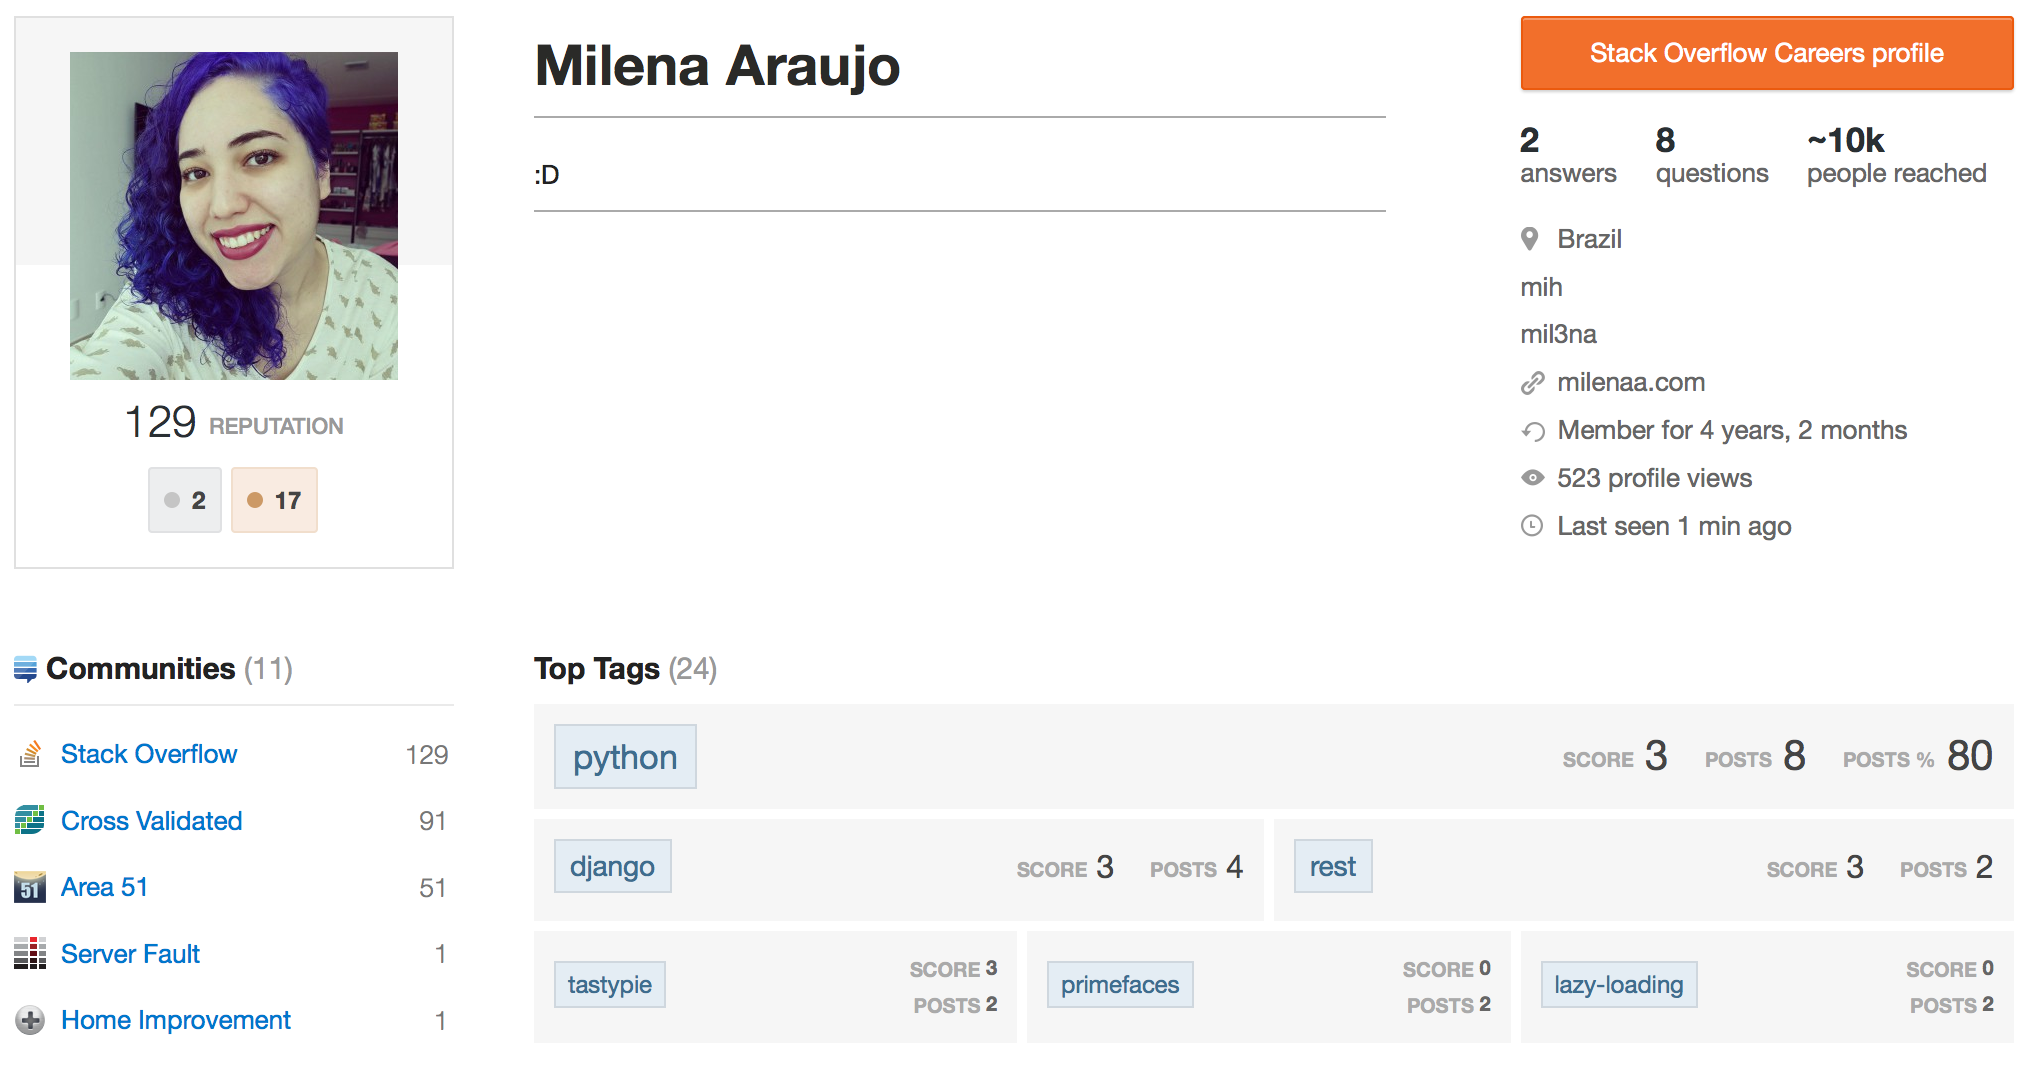
\includegraphics[width=1\columnwidth]{figures/user.png}
  \caption[Perfil de um usuário cadastrado]{Perfil de um usuário cadastrado.}~\label{fig:user-reg}
\end{figure}

Os votos são o meio que o \emph{StackExchange} usa para permitir que a própria comunidade mantenha a qualidade das contribuições. Para isso, eles são restritos aos usuários registrados. Os que possuem uma reputação de 15 pontos ou mais podem votar afirmando que uma contribuição é boa. Apenas aqueles usuários com 125 pontos ou mais podem votar afirmando que uma contribuição é ruim. Restringindo assim aos usuários que já participaram do site ou da plataforma o controle de qualidade do conteúdo do site.
% Estrutura de perguntas e respostas do SE
% Sistema de qualidade

Uma particularidade da plataforma StackExchange é que, em seus sites, o anonimato do usuário é respeitado e preservado. Primeiramente, apesar da plataforma sugerir que o usuário preencha uma vasta quantidade de informações pessoais ao se cadastrar, apenas o seu \emph{email} e nome de usuário (que pode ser gerado automaticamente) são obrigatórios. Por decisão interna, o gênero do usuário não é incluso dentre as informações pessoais que um usuário pode inserir em seu perfil.

Ademais, um usuário não precisa estar cadastrado para participar dos sites. Qualquer pessoa pode responder a qualquer pergunta aberta (que ainda possa receber respostas). Um perfil temporário é criado para este usuário e não pode mais ser acessado pelo mesmo após sua sessão expirar. Tal perfil é marcado como "não registrado". Um exemplo pode ser encontrado na Figura~\ref{fig:user-not-reg}.

Apesar da vantagem da anonimidade, estes usuários que optaram por não se cadastrar não poderão usufruir das regalias que os usuários cadastrados que participam da comunidade possuem. Poder contribuir com perguntas e comentários, ter uma reputação associada ao seu nome e poder, caso tenha reputação suficiente, participar do processo de avaliação de qualidade do conteúdo do site, são alguns exemplos de habilidades restritas aos usuários cadastrados.

\begin{figure}[!b]
  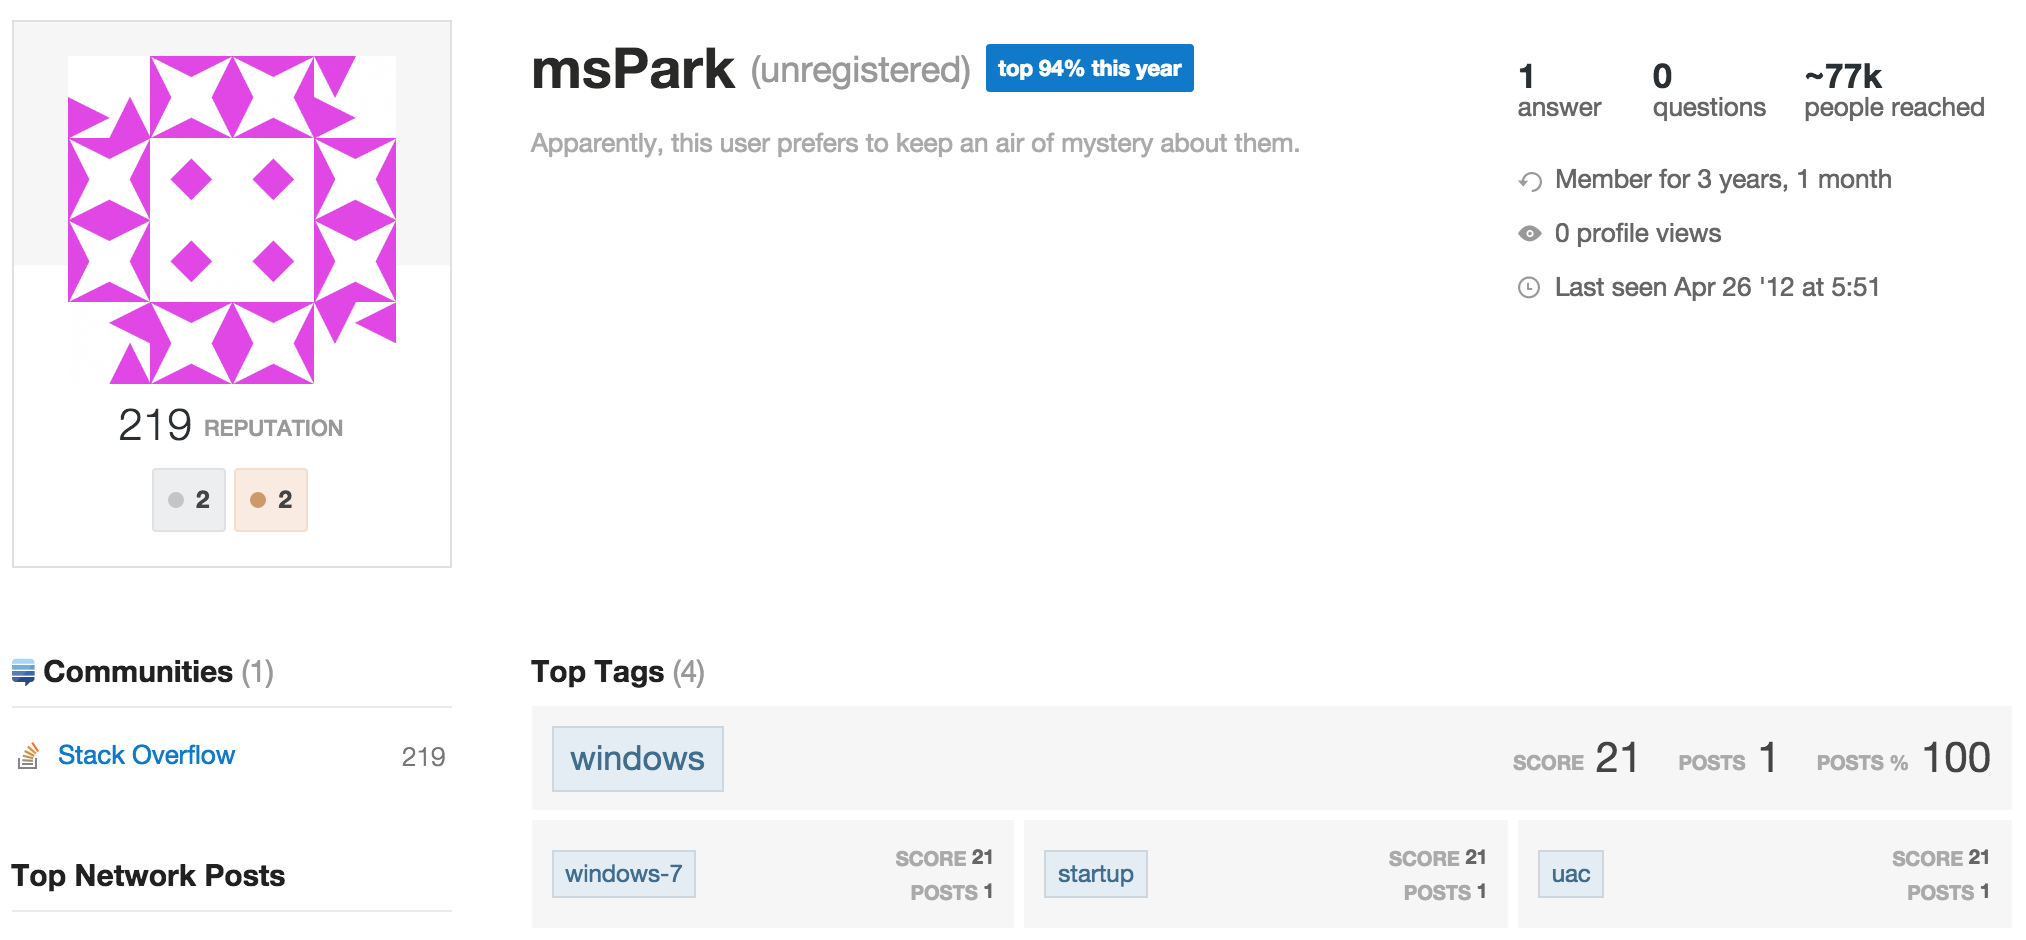
\includegraphics[width=1\columnwidth]{figures/user3.png}
  \caption[Perfil de um usuário não cadastrado]{Perfil de um usuário não cadastrado. É criado um perfil temporário que não pode mais ser acessado pelo usuário após o término da sessão.}~\label{fig:user-not-reg}
\end{figure}



% É necessário estar cadastrado para perguntar, perfil temporário para respostas
% Perfil dos usuários
% Não obrigatoriedade de cadastro
% falta de gênero, campos opcionais





% subsubsection modo_de_funcionamento (end)

